\subsection{Датасет Visible Human Project}

В качестве цели визуализации выбран датасет Visible Human Project \cite{ackerman1999visible}, а точнее его часть с мужским телом. Донором для датасета является Джозеф Пол Джерниган, 38 летний заключенный, казненный в 1993 году. Он завещал своё тело науке. Благодаря нему собраны следующие данные:
\begin{itemize}
	\item Около 500 МРТ снимков с шагом $4$ мм разрешения $256\times256$ (размер пикселя $1.88$ мм), каждый воксель кодируется одним скалярным значением с точностью $12$ бит;
	\item Фотографии срезов замороженного тела с шагом $1$ мм разрешения $2048\times1216$ (что соответствует размеру пикслеля в $0.33$ мм), итого: 1871 срезов, каждый воксель кодируется 24 битами (по 8 на канал RGB);
	\item Компьютерная томография с шагом $1$ мм (соотвествует цветным изображениям) разрешения $512\times512$ (размер пикселя $1$ мм) с 12 битным кодированием.
\end{itemize}

В работе же используется его обработанная версия \cite{segmented_vhp}, содержащая к сожалению только туловище, характеристики этих данных следующие:
\begin{itemize}
	\item Обработаны КТ и цветные среды (рис. \ref{fig:vhp}), между ними теперь есть однозначное соответствие, их размер стал $573\times330\times774$, а воксель теперь кубический со стороной $1$ мм (в отличие от анизотропного пикселя $0.33\times0.33\times1$ мм для цветных изображений из оригинального датасета), кодирование КТ нормализовано и записано в $8$ битном формате;
	\item Каждый воксель этой воксельной сетки сегментирован; был написан скрипт, который извлекает информацию об описании каждой метки, он приведен в листинге \ref{lst:labels-to-json}.
\end{itemize}

Метки и их описания приведены в листинге \ref{lst:labels-json}.

\begin{figure}[ht]
	\centering
	\begin{subfigure}[b]{0.39\textwidth}
		\centering
		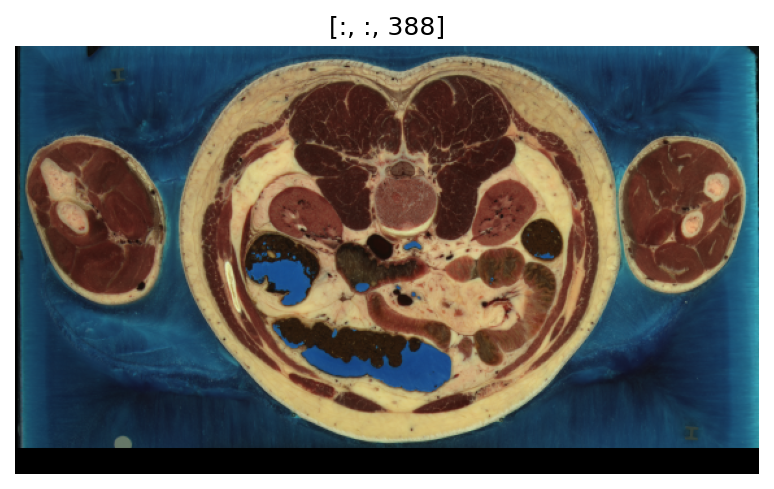
\includegraphics[width=\textwidth, height=8cm, keepaspectratio]{assets/VHP_ZSlice.png}
		\caption{388-е исходное изображение \\ (слайс вдоль $Oxy$)}
	\end{subfigure}%
	\hfill
	\begin{subfigure}[b]{0.39\textwidth}
		\centering
		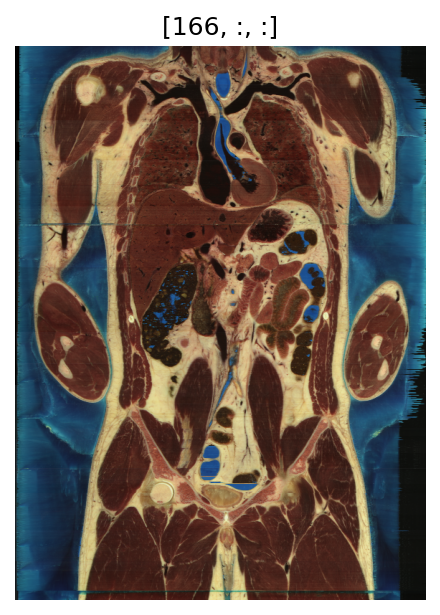
\includegraphics[width=\textwidth, height=8cm, keepaspectratio]{assets/VHP_XSlice.png}
		\caption{166-й слайс по ширине \\ (вдоль $Oyz$)}
	\end{subfigure}%
	\hfill
	\begin{subfigure}[b]{0.22\textwidth}
		\centering
		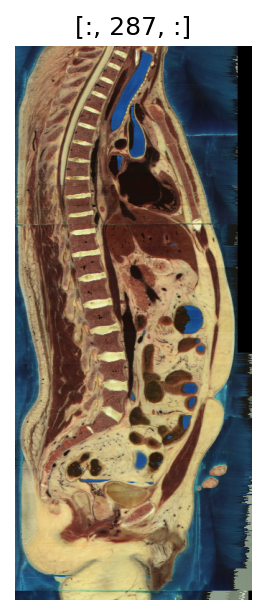
\includegraphics[width=\textwidth, height=8cm, keepaspectratio]{assets/VHP_YSlice.png}
		\caption{287-й слайс \\ по высоте ($Oxz$)}
	\end{subfigure}
	\caption{Слайсы по разным пространством. Слева --- одно из исходных изображения датасета, по центру и справа получены сложением всех изображений в стопку и срезом вдоль других плоскостей}
	\label{fig:vhp}
\end{figure}

Из датасета в качестве визуализации выбрана костная система человека, как самая наглядная и покрывающая всё туловище. Код вместе с метками, соответствующими костям, приведен в листинге \ref{lst:raw-to-skeletal}.